% Drawing 58/04-6 -- folder 58, batch 04, archive page 65 (PDF page 66).
% Transcription: marge gauche, en bas : un cercle épais barré d'un gros trait oblique portant un point ; plus bas, un petit carré pointé, en perspective, dans un cadre en spirale.
% Kind: circle with a heavy stroke through a point; a pointed square in a frame. Method 2 (schematic redraw from the facsimile). Status: partial.
% Notes: Top: a heavy upright oval crossed by a heavy oblique stroke which carries a point at the centre. Bottom: a small quadrilateral (a square seen aslant) with a point at its centre and a short stroke rising from its upper left corner, inside a frame drawn in one spiral stroke (left side, bottom, then top, right side and back under the square). Still differs: the frame is a free spiral, drawn through points read on the crop; a stroke under the square (from its left to below its right corner) is drawn as one line. Redrawn 2026-11-12 (issue 128): to check again.
% Coordinates: 1 unit = 0.7 mm = 1/100 of the crop width (bbox in page fractions: [0.14, 0.62, 0.34, 0.81]).
% Redrawn by Claude (claude-fable-5-2), issue #128, 2026-11-12; not checked by a human; not compiled (no TeX in the session).
% Rights: reproduces part of the work -- behind RENDER_TRANSCRIPTS, never published by itself.
\documentclass[tikz,border=3pt]{standalone}
\usepackage{amsmath,amssymb}
\usetikzlibrary{patterns,arrows.meta}
\tikzset{pencil/.style={black!45}, struck/.style={black!35}, mpt/.style={circle,draw,inner sep=1.3pt}, pt/.style={circle,fill,inner sep=0.9pt}, opt/.style={circle,draw,fill=white,inner sep=1.1pt}}
\begin{document}
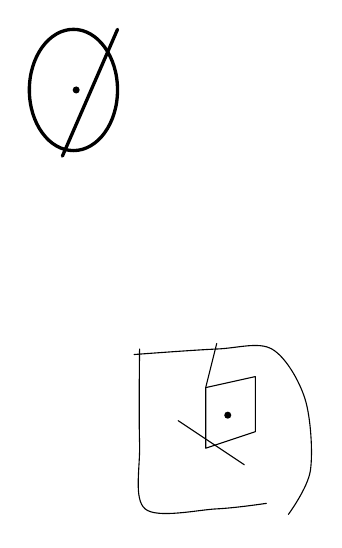
\begin{tikzpicture}[x=0.7mm,y=0.7mm,line cap=round,line join=round,font=\scriptsize]
\draw[very thick] (29,-36) ellipse[x radius=8, y radius=11];
\draw[very thick] (37,-25) -- (27,-48);
\node[pt] at (29.5,-36) {};
\draw (53,-90) -- (62,-88) -- (62,-98) -- (53,-101) -- cycle;
\node[pt] at (57,-95) {};
\draw (55,-82) -- (53,-90);
\draw (48,-96) -- (60,-104);
\draw plot[smooth, tension=0.55] coordinates {(41,-83) (41,-100) (42,-112) (55,-112) (64,-111)};
\draw plot[smooth, tension=0.55] coordinates {(40,-84) (55,-83) (65,-83) (71,-92) (72,-105) (68,-113)};
\end{tikzpicture}
\end{document}
